\documentclass[12pt, a4paper]{article}
% \usepackage[spanish]{babel}
% \usepackage{lipsum}
% \usepackage{natbib}
% \usepackage{graphicx}
\usepackage{analysis_orax}
\usepackage{tikz}


% \usepackage[utf8]{vietnam}

\usepackage{indentfirst}
\setlength{\parindent}{1cm}

\usepackage{enumerate}
\usepackage{enumitem}
% \renewcommand{\labelenumi}{{\bf Câu \arabic{enumi}:\\}}
% Các gói toán
\usepackage{amsmath}
\usepackage{amssymb}
\usepackage{amsthm}

% \usepackage{fourier}
\usepackage{mathtools}
% \usepackage{cleveref}

\usepackage{listings}
\usepackage{draftwatermark}
% tùy chỉnh watermark
\SetWatermarkText{Vũ Huy} %chữ ký chìm
\SetWatermarkScale{0.5}
\SetWatermarkAngle{35} % độ nghiêng, để mặc định là 45 độ
\SetWatermarkColor{red!5} %màu, !15 là độ đậm nhạt 15%
\SetWatermarkFontSize{10cm}




\begin{document}
% \section{Analysis Report}
% \subsection{Subtitle}

\begin{center}
    \textbf{VIỆN TOÁN ỨNG DỤNG VÀ TIN HỌC}\\
    \textbf{TRƯỜNG ĐẠI HỌC BÁCH KHOA HÀ NỘI}\\
    ==========***==========
    \\ \textbf{ĐỀ THI CUỐI KỲ 20221\\
    MÔN: TOÁN RỜI RẠC, THỜI GIAN: 90 PHÚT\\ ==========***==========\\ ĐỀ 2}
\end{center}
\indent \textbf{Họ và tên:} \hspace{10cm}\textbf{Mã sinh viên:}

\begin{enumerate}[label = {\bf Câu \arabic*.}]
    \item Cho M là tập các số tự nhiên chẵn. Hỏi tập E = M $\times$ M(Tích đề các) có phải là tập đếm được không. Giải thích?
    
    \item Cho A = $\{1, 4, 6, 7, 10, 12, 13, 16, 24, 27\}.$ Xét 1 hệ $\mathbb{R}$ trong A nhau sau $\forall x, y \thickspace \in A$, x $\mathbb{R}$ y $\Leftrightarrow$ $3x+4 \thickspace \vdots\thickspace 4$
    \begin{enumerate}[label = \alph*)]
        \item Chứng minh $\mathbb{R}$ là một quan hệ tương đương trên A
        \item Tìm lớp tương đương của phần tử 1
    \end{enumerate}

    \item Cho hình vuông có độ dài mỗi cạnh là 6. Hỏi phải đặt trong hình vuông ít nhất bao nhiêu điểm để sao cho luôn chỉ ra được ít nhất 2 điểm mà khoảng cách của chúng không vượt quá $2\sqrt{2}$

    \item Có bao nhiêu chuỗi nhị phân có độ dài 8 bits hoặc chứa 3 bits 0 liên tiếp hoặc chứa 2 bits 1 liên tiếp.

    \item Cho đồ thị G như hình:
    \begin{center}
        

\tikzset{every picture/.style={line width=0.75pt}} %set default line width to 0.75pt        

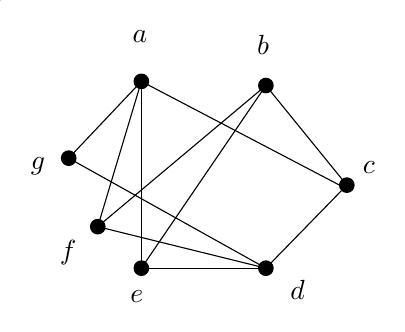
\begin{tikzpicture}[x=0.75pt,y=0.75pt,yscale=-1,xscale=1]
%uncomment if require: \path (0,300); %set diagram left start at 0, and has height of 300

%Shape: Circle [id:dp6391804589617953] 
\draw  [fill={rgb, 255:red, 0; green, 0; blue, 0 }  ,fill opacity=1 ] (102,146) .. controls (102,144.07) and (103.57,142.5) .. (105.5,142.5) .. controls (107.43,142.5) and (109,144.07) .. (109,146) .. controls (109,147.93) and (107.43,149.5) .. (105.5,149.5) .. controls (103.57,149.5) and (102,147.93) .. (102,146) -- cycle ;
%Shape: Circle [id:dp8175285810366237] 
\draw  [fill={rgb, 255:red, 0; green, 0; blue, 0 }  ,fill opacity=1 ] (137,109) .. controls (137,107.07) and (138.57,105.5) .. (140.5,105.5) .. controls (142.43,105.5) and (144,107.07) .. (144,109) .. controls (144,110.93) and (142.43,112.5) .. (140.5,112.5) .. controls (138.57,112.5) and (137,110.93) .. (137,109) -- cycle ;
%Shape: Circle [id:dp1771585203526609] 
\draw  [fill={rgb, 255:red, 0; green, 0; blue, 0 }  ,fill opacity=1 ] (197,111) .. controls (197,109.07) and (198.57,107.5) .. (200.5,107.5) .. controls (202.43,107.5) and (204,109.07) .. (204,111) .. controls (204,112.93) and (202.43,114.5) .. (200.5,114.5) .. controls (198.57,114.5) and (197,112.93) .. (197,111) -- cycle ;
%Shape: Circle [id:dp6518377302295517] 
\draw  [fill={rgb, 255:red, 0; green, 0; blue, 0 }  ,fill opacity=1 ] (197,199) .. controls (197,197.07) and (198.57,195.5) .. (200.5,195.5) .. controls (202.43,195.5) and (204,197.07) .. (204,199) .. controls (204,200.93) and (202.43,202.5) .. (200.5,202.5) .. controls (198.57,202.5) and (197,200.93) .. (197,199) -- cycle ;
%Shape: Circle [id:dp014727044231518382] 
\draw  [fill={rgb, 255:red, 0; green, 0; blue, 0 }  ,fill opacity=1 ] (116,179) .. controls (116,177.07) and (117.57,175.5) .. (119.5,175.5) .. controls (121.43,175.5) and (123,177.07) .. (123,179) .. controls (123,180.93) and (121.43,182.5) .. (119.5,182.5) .. controls (117.57,182.5) and (116,180.93) .. (116,179) -- cycle ;
%Shape: Circle [id:dp45243107582265263] 
\draw  [fill={rgb, 255:red, 0; green, 0; blue, 0 }  ,fill opacity=1 ] (137,199) .. controls (137,197.07) and (138.57,195.5) .. (140.5,195.5) .. controls (142.43,195.5) and (144,197.07) .. (144,199) .. controls (144,200.93) and (142.43,202.5) .. (140.5,202.5) .. controls (138.57,202.5) and (137,200.93) .. (137,199) -- cycle ;
%Shape: Circle [id:dp23815426410166096] 
\draw  [fill={rgb, 255:red, 0; green, 0; blue, 0 }  ,fill opacity=1 ] (236,159) .. controls (236,157.07) and (237.57,155.5) .. (239.5,155.5) .. controls (241.43,155.5) and (243,157.07) .. (243,159) .. controls (243,160.93) and (241.43,162.5) .. (239.5,162.5) .. controls (237.57,162.5) and (236,160.93) .. (236,159) -- cycle ;
%Straight Lines [id:da7992163569841868] 
\draw    (105.5,146) -- (140.5,109) ;
%Straight Lines [id:da824234465217542] 
\draw    (119.5,179) -- (200.5,199) ;
%Straight Lines [id:da250994642568104] 
\draw    (200.5,111) -- (239.5,159) ;
%Straight Lines [id:da046990899098223515] 
\draw    (140.5,109) -- (236,159) ;
%Straight Lines [id:da6741191771794801] 
\draw    (119.5,179) -- (140.5,109) ;
%Straight Lines [id:da5194715327790833] 
\draw    (119.5,179) -- (200.5,111) ;
%Straight Lines [id:da9492114188424601] 
\draw    (105.5,146) -- (200.5,199) ;
%Straight Lines [id:da7302489664041212] 
\draw    (140.5,199) -- (200.5,111) ;
%Straight Lines [id:da572824221337896] 
\draw    (140.5,199) -- (200.5,199) ;
%Straight Lines [id:da9800786990913697] 
\draw    (200.5,199) -- (239.5,159) ;
%Straight Lines [id:da3192315828453116] 
\draw    (140.5,109) -- (140.5,199) ;

% Text Node
\draw (211,203.4) node [anchor=north west][inner sep=0.75pt]    {$d$};
% Text Node
\draw (134,208.4) node [anchor=north west][inner sep=0.75pt]    {$e$};
% Text Node
\draw (86,144.4) node [anchor=north west][inner sep=0.75pt]    {$g$};
% Text Node
\draw (100,184.4) node [anchor=north west][inner sep=0.75pt]    {$f$};
% Text Node
\draw (135,83.4) node [anchor=north west][inner sep=0.75pt]    {$a$};
% Text Node
\draw (195,85.4) node [anchor=north west][inner sep=0.75pt]    {$b$};
% Text Node
\draw (246,146.4) node [anchor=north west][inner sep=0.75pt]    {$c$};


\end{tikzpicture}
    \end{center}
    \begin{enumerate}[label = \alph*)]
        \item $\Delta(G), \delta(G)$
        \item Độ lệch tâm các đỉnh
    \end{enumerate}
    \item Cho đồ thị G 
    \begin{center}
        

\tikzset{every picture/.style={line width=0.75pt}} %set default line width to 0.75pt        

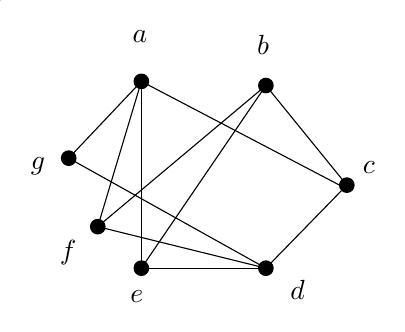
\begin{tikzpicture}[x=0.75pt,y=0.75pt,yscale=-1,xscale=1]
%uncomment if require: \path (0,300); %set diagram left start at 0, and has height of 300

%Shape: Circle [id:dp6391804589617953] 
\draw  [fill={rgb, 255:red, 0; green, 0; blue, 0 }  ,fill opacity=1 ] (102,146) .. controls (102,144.07) and (103.57,142.5) .. (105.5,142.5) .. controls (107.43,142.5) and (109,144.07) .. (109,146) .. controls (109,147.93) and (107.43,149.5) .. (105.5,149.5) .. controls (103.57,149.5) and (102,147.93) .. (102,146) -- cycle ;
%Shape: Circle [id:dp8175285810366237] 
\draw  [fill={rgb, 255:red, 0; green, 0; blue, 0 }  ,fill opacity=1 ] (137,109) .. controls (137,107.07) and (138.57,105.5) .. (140.5,105.5) .. controls (142.43,105.5) and (144,107.07) .. (144,109) .. controls (144,110.93) and (142.43,112.5) .. (140.5,112.5) .. controls (138.57,112.5) and (137,110.93) .. (137,109) -- cycle ;
%Shape: Circle [id:dp1771585203526609] 
\draw  [fill={rgb, 255:red, 0; green, 0; blue, 0 }  ,fill opacity=1 ] (197,111) .. controls (197,109.07) and (198.57,107.5) .. (200.5,107.5) .. controls (202.43,107.5) and (204,109.07) .. (204,111) .. controls (204,112.93) and (202.43,114.5) .. (200.5,114.5) .. controls (198.57,114.5) and (197,112.93) .. (197,111) -- cycle ;
%Shape: Circle [id:dp6518377302295517] 
\draw  [fill={rgb, 255:red, 0; green, 0; blue, 0 }  ,fill opacity=1 ] (197,199) .. controls (197,197.07) and (198.57,195.5) .. (200.5,195.5) .. controls (202.43,195.5) and (204,197.07) .. (204,199) .. controls (204,200.93) and (202.43,202.5) .. (200.5,202.5) .. controls (198.57,202.5) and (197,200.93) .. (197,199) -- cycle ;
%Shape: Circle [id:dp014727044231518382] 
\draw  [fill={rgb, 255:red, 0; green, 0; blue, 0 }  ,fill opacity=1 ] (116,179) .. controls (116,177.07) and (117.57,175.5) .. (119.5,175.5) .. controls (121.43,175.5) and (123,177.07) .. (123,179) .. controls (123,180.93) and (121.43,182.5) .. (119.5,182.5) .. controls (117.57,182.5) and (116,180.93) .. (116,179) -- cycle ;
%Shape: Circle [id:dp45243107582265263] 
\draw  [fill={rgb, 255:red, 0; green, 0; blue, 0 }  ,fill opacity=1 ] (137,199) .. controls (137,197.07) and (138.57,195.5) .. (140.5,195.5) .. controls (142.43,195.5) and (144,197.07) .. (144,199) .. controls (144,200.93) and (142.43,202.5) .. (140.5,202.5) .. controls (138.57,202.5) and (137,200.93) .. (137,199) -- cycle ;
%Shape: Circle [id:dp23815426410166096] 
\draw  [fill={rgb, 255:red, 0; green, 0; blue, 0 }  ,fill opacity=1 ] (236,159) .. controls (236,157.07) and (237.57,155.5) .. (239.5,155.5) .. controls (241.43,155.5) and (243,157.07) .. (243,159) .. controls (243,160.93) and (241.43,162.5) .. (239.5,162.5) .. controls (237.57,162.5) and (236,160.93) .. (236,159) -- cycle ;
%Straight Lines [id:da7992163569841868] 
\draw    (105.5,146) -- (140.5,109) ;
%Straight Lines [id:da824234465217542] 
\draw    (119.5,179) -- (200.5,199) ;
%Straight Lines [id:da250994642568104] 
\draw    (200.5,111) -- (239.5,159) ;
%Straight Lines [id:da046990899098223515] 
\draw    (140.5,109) -- (236,159) ;
%Straight Lines [id:da6741191771794801] 
\draw    (119.5,179) -- (140.5,109) ;
%Straight Lines [id:da5194715327790833] 
\draw    (119.5,179) -- (200.5,111) ;
%Straight Lines [id:da9492114188424601] 
\draw    (105.5,146) -- (200.5,199) ;
%Straight Lines [id:da7302489664041212] 
\draw    (140.5,199) -- (200.5,111) ;
%Straight Lines [id:da572824221337896] 
\draw    (140.5,199) -- (200.5,199) ;
%Straight Lines [id:da9800786990913697] 
\draw    (200.5,199) -- (239.5,159) ;
%Straight Lines [id:da3192315828453116] 
\draw    (140.5,109) -- (140.5,199) ;

% Text Node
\draw (211,203.4) node [anchor=north west][inner sep=0.75pt]    {$d$};
% Text Node
\draw (134,208.4) node [anchor=north west][inner sep=0.75pt]    {$e$};
% Text Node
\draw (86,144.4) node [anchor=north west][inner sep=0.75pt]    {$g$};
% Text Node
\draw (100,184.4) node [anchor=north west][inner sep=0.75pt]    {$f$};
% Text Node
\draw (135,83.4) node [anchor=north west][inner sep=0.75pt]    {$a$};
% Text Node
\draw (195,85.4) node [anchor=north west][inner sep=0.75pt]    {$b$};
% Text Node
\draw (246,146.4) node [anchor=north west][inner sep=0.75pt]    {$c$};


\end{tikzpicture}
    \end{center}
    \begin{enumerate}[label = \alph*)]
        \item $G$ có phải đồ thị 2 phía không? Giải thích?
        \item Xác định $\kappa(G)$
    \end{enumerate}

    \item Trình bày thuật toán Dijkstra tìm độ dài đường đi ngắn nhất từ "a" đến các đỉnh còn lại
        \begin{center}


\tikzset{every picture/.style={line width=0.75pt}} %set default line width to 0.75pt        

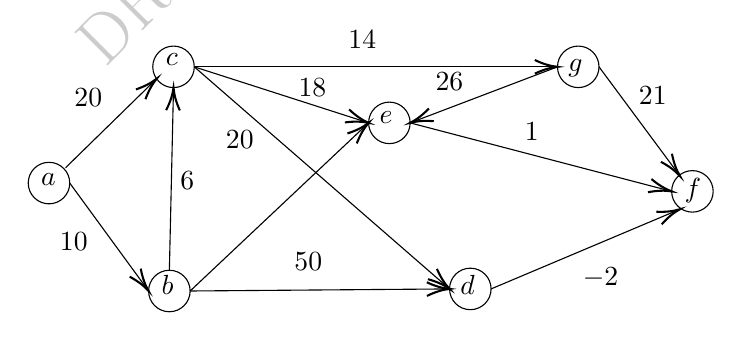
\begin{tikzpicture}[x=0.75pt,y=0.75pt,yscale=-1,xscale=1]
%uncomment if require: \path (0,300); %set diagram left start at 0, and has height of 300

%Shape: Circle [id:dp21282070709112233] 
\draw   (100,157) .. controls (100,151.48) and (104.48,147) .. (110,147) .. controls (115.52,147) and (120,151.48) .. (120,157) .. controls (120,162.52) and (115.52,167) .. (110,167) .. controls (104.48,167) and (100,162.52) .. (100,157) -- cycle ;
%Shape: Circle [id:dp3191227487357018] 
\draw   (160,101) .. controls (160,95.48) and (164.48,91) .. (170,91) .. controls (175.52,91) and (180,95.48) .. (180,101) .. controls (180,106.52) and (175.52,111) .. (170,111) .. controls (164.48,111) and (160,106.52) .. (160,101) -- cycle ;
%Shape: Circle [id:dp68041019373638] 
\draw   (158,209) .. controls (158,203.48) and (162.48,199) .. (168,199) .. controls (173.52,199) and (178,203.48) .. (178,209) .. controls (178,214.52) and (173.52,219) .. (168,219) .. controls (162.48,219) and (158,214.52) .. (158,209) -- cycle ;
%Shape: Circle [id:dp08981107421631718] 
\draw   (303,208) .. controls (303,202.48) and (307.48,198) .. (313,198) .. controls (318.52,198) and (323,202.48) .. (323,208) .. controls (323,213.52) and (318.52,218) .. (313,218) .. controls (307.48,218) and (303,213.52) .. (303,208) -- cycle ;
%Shape: Circle [id:dp24991413932590145] 
\draw   (264,128) .. controls (264,122.48) and (268.48,118) .. (274,118) .. controls (279.52,118) and (284,122.48) .. (284,128) .. controls (284,133.52) and (279.52,138) .. (274,138) .. controls (268.48,138) and (264,133.52) .. (264,128) -- cycle ;
%Shape: Circle [id:dp7235474855555515] 
\draw   (355,101) .. controls (355,95.48) and (359.48,91) .. (365,91) .. controls (370.52,91) and (375,95.48) .. (375,101) .. controls (375,106.52) and (370.52,111) .. (365,111) .. controls (359.48,111) and (355,106.52) .. (355,101) -- cycle ;
%Shape: Circle [id:dp5926071070272325] 
\draw   (410,161) .. controls (410,155.48) and (414.48,151) .. (420,151) .. controls (425.52,151) and (430,155.48) .. (430,161) .. controls (430,166.52) and (425.52,171) .. (420,171) .. controls (414.48,171) and (410,166.52) .. (410,161) -- cycle ;
%Straight Lines [id:da6973607404332958] 
\draw    (118,149.6) -- (160.57,108) ;
\draw [shift={(162,106.6)}, rotate = 135.66] [color={rgb, 255:red, 0; green, 0; blue, 0 }  ][line width=0.75]    (10.93,-3.29) .. controls (6.95,-1.4) and (3.31,-0.3) .. (0,0) .. controls (3.31,0.3) and (6.95,1.4) .. (10.93,3.29)   ;
%Straight Lines [id:da2440041361675862] 
\draw    (168,199) -- (169.95,113) ;
\draw [shift={(170,111)}, rotate = 91.3] [color={rgb, 255:red, 0; green, 0; blue, 0 }  ][line width=0.75]    (10.93,-3.29) .. controls (6.95,-1.4) and (3.31,-0.3) .. (0,0) .. controls (3.31,0.3) and (6.95,1.4) .. (10.93,3.29)   ;
%Straight Lines [id:da9296282512589156] 
\draw    (180,101) -- (353,101) ;
\draw [shift={(355,101)}, rotate = 180] [color={rgb, 255:red, 0; green, 0; blue, 0 }  ][line width=0.75]    (10.93,-3.29) .. controls (6.95,-1.4) and (3.31,-0.3) .. (0,0) .. controls (3.31,0.3) and (6.95,1.4) .. (10.93,3.29)   ;
%Straight Lines [id:da47089328440362] 
\draw    (375,101) -- (412.81,151.99) ;
\draw [shift={(414,153.6)}, rotate = 233.45] [color={rgb, 255:red, 0; green, 0; blue, 0 }  ][line width=0.75]    (10.93,-3.29) .. controls (6.95,-1.4) and (3.31,-0.3) .. (0,0) .. controls (3.31,0.3) and (6.95,1.4) .. (10.93,3.29)   ;
%Straight Lines [id:da9958580195610556] 
\draw    (120,157) -- (156.82,207.39) ;
\draw [shift={(158,209)}, rotate = 233.84] [color={rgb, 255:red, 0; green, 0; blue, 0 }  ][line width=0.75]    (10.93,-3.29) .. controls (6.95,-1.4) and (3.31,-0.3) .. (0,0) .. controls (3.31,0.3) and (6.95,1.4) .. (10.93,3.29)   ;
%Straight Lines [id:da1763229454038353] 
\draw    (178,209) -- (301,208.02) ;
\draw [shift={(303,208)}, rotate = 179.54] [color={rgb, 255:red, 0; green, 0; blue, 0 }  ][line width=0.75]    (10.93,-3.29) .. controls (6.95,-1.4) and (3.31,-0.3) .. (0,0) .. controls (3.31,0.3) and (6.95,1.4) .. (10.93,3.29)   ;
%Straight Lines [id:da721480543591394] 
\draw    (180,101) -- (301.49,206.69) ;
\draw [shift={(303,208)}, rotate = 221.02] [color={rgb, 255:red, 0; green, 0; blue, 0 }  ][line width=0.75]    (10.93,-3.29) .. controls (6.95,-1.4) and (3.31,-0.3) .. (0,0) .. controls (3.31,0.3) and (6.95,1.4) .. (10.93,3.29)   ;
%Straight Lines [id:da2921022227107104] 
\draw    (178,209) -- (262.54,129.37) ;
\draw [shift={(264,128)}, rotate = 136.71] [color={rgb, 255:red, 0; green, 0; blue, 0 }  ][line width=0.75]    (10.93,-3.29) .. controls (6.95,-1.4) and (3.31,-0.3) .. (0,0) .. controls (3.31,0.3) and (6.95,1.4) .. (10.93,3.29)   ;
%Straight Lines [id:da8650578711670842] 
\draw    (180,101) -- (262.1,127.39) ;
\draw [shift={(264,128)}, rotate = 197.82] [color={rgb, 255:red, 0; green, 0; blue, 0 }  ][line width=0.75]    (10.93,-3.29) .. controls (6.95,-1.4) and (3.31,-0.3) .. (0,0) .. controls (3.31,0.3) and (6.95,1.4) .. (10.93,3.29)   ;
%Straight Lines [id:da23500910017137344] 
\draw    (323,208) -- (412.16,170.38) ;
\draw [shift={(414,169.6)}, rotate = 157.12] [color={rgb, 255:red, 0; green, 0; blue, 0 }  ][line width=0.75]    (10.93,-3.29) .. controls (6.95,-1.4) and (3.31,-0.3) .. (0,0) .. controls (3.31,0.3) and (6.95,1.4) .. (10.93,3.29)   ;
%Straight Lines [id:da1699593288389596] 
\draw    (284,128) -- (408.07,160.49) ;
\draw [shift={(410,161)}, rotate = 194.68] [color={rgb, 255:red, 0; green, 0; blue, 0 }  ][line width=0.75]    (10.93,-3.29) .. controls (6.95,-1.4) and (3.31,-0.3) .. (0,0) .. controls (3.31,0.3) and (6.95,1.4) .. (10.93,3.29)   ;
%Straight Lines [id:da6876101980317786] 
\draw    (355,101) -- (285.87,127.29) ;
\draw [shift={(284,128)}, rotate = 339.18] [color={rgb, 255:red, 0; green, 0; blue, 0 }  ][line width=0.75]    (10.93,-3.29) .. controls (6.95,-1.4) and (3.31,-0.3) .. (0,0) .. controls (3.31,0.3) and (6.95,1.4) .. (10.93,3.29)   ;

% Text Node
\draw (105,151.4) node [anchor=north west][inner sep=0.75pt]    {$a$};
% Text Node
\draw (165,93.4) node [anchor=north west][inner sep=0.75pt]    {$c$};
% Text Node
\draw (268,121.4) node [anchor=north west][inner sep=0.75pt]    {$e$};
% Text Node
\draw (163,200.4) node [anchor=north west][inner sep=0.75pt]    {$b$};
% Text Node
\draw (307,200.4) node [anchor=north west][inner sep=0.75pt]    {$d$};
% Text Node
\draw (359,96.4) node [anchor=north west][inner sep=0.75pt]    {$g$};
% Text Node
\draw (415,153.4) node [anchor=north west][inner sep=0.75pt]    {$f$};
% Text Node
\draw (114,179.4) node [anchor=north west][inner sep=0.75pt]    {$10$};
% Text Node
\draw (121,110.4) node [anchor=north west][inner sep=0.75pt]    {$20$};
% Text Node
\draw (253,82.4) node [anchor=north west][inner sep=0.75pt]    {$14$};
% Text Node
\draw (393,109.4) node [anchor=north west][inner sep=0.75pt]    {$21$};
% Text Node
\draw (366,196.4) node [anchor=north west][inner sep=0.75pt]    {$-2$};
% Text Node
\draw (172,150.4) node [anchor=north west][inner sep=0.75pt]    {$6$};
% Text Node
\draw (227,189.4) node [anchor=north west][inner sep=0.75pt]    {$50$};
% Text Node
\draw (338,126.4) node [anchor=north west][inner sep=0.75pt]    {$1$};
% Text Node
\draw (295,102.4) node [anchor=north west][inner sep=0.75pt]    {$26$};
% Text Node
\draw (229,105.4) node [anchor=north west][inner sep=0.75pt]    {$18$};
% Text Node
\draw (194,130.4) node [anchor=north west][inner sep=0.75pt]    {$20$};


\end{tikzpicture}
        \end{center}
    \item Tìm tất cả đơn đồ thị G, không đẳng cấu, chứa 3 thành phần liên thông $G_1, \thickspace G_2, \thickspace G_3$ thỏa mãn $m(G) = 13,\thickspace n(G) = 10$ và
    \begin{itemize}
        \item[i)] $G_1, \thickspace G_2$ không đẳng cấu
        \item[ii)] $L(G_1)$ và $L(G_2)$ đẳng cấu, ở đó $L(G_i)$ là đồ thị đường của $G_i$
        \item[iii)] $G_3$ là cây có chính xác 3 lá
   \end{itemize}
   \item Hai đồ thị sau có đẳng cấu không? Giải thích?
    \begin{center}
        

\tikzset{every picture/.style={line width=0.75pt}} %set default line width to 0.75pt        

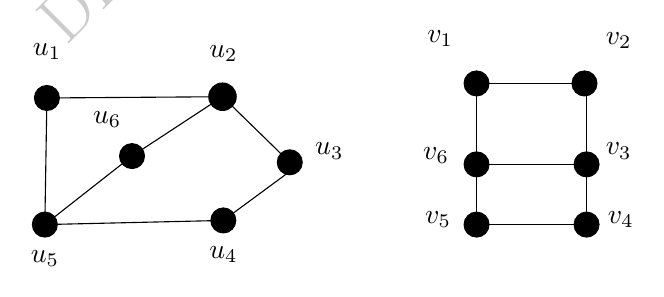
\begin{tikzpicture}[x=0.75pt,y=0.75pt,yscale=-1,xscale=1]
%uncomment if require: \path (0,300); %set diagram left start at 0, and has height of 300

%Shape: Circle [id:dp590335671374441] 
\draw  [fill={rgb, 255:red, 0; green, 0; blue, 0 }  ,fill opacity=1 ] (141,114) .. controls (141,110.69) and (143.69,108) .. (147,108) .. controls (150.31,108) and (153,110.69) .. (153,114) .. controls (153,117.31) and (150.31,120) .. (147,120) .. controls (143.69,120) and (141,117.31) .. (141,114) -- cycle ;
%Shape: Circle [id:dp623505284238898] 
\draw  [fill={rgb, 255:red, 0; green, 0; blue, 0 }  ,fill opacity=1 ] (225,113.4) .. controls (225,109.75) and (227.95,106.8) .. (231.6,106.8) .. controls (235.25,106.8) and (238.2,109.75) .. (238.2,113.4) .. controls (238.2,117.05) and (235.25,120) .. (231.6,120) .. controls (227.95,120) and (225,117.05) .. (225,113.4) -- cycle ;
%Shape: Circle [id:dp7399847996591435] 
\draw  [fill={rgb, 255:red, 0; green, 0; blue, 0 }  ,fill opacity=1 ] (226,173) .. controls (226,169.69) and (228.69,167) .. (232,167) .. controls (235.31,167) and (238,169.69) .. (238,173) .. controls (238,176.31) and (235.31,179) .. (232,179) .. controls (228.69,179) and (226,176.31) .. (226,173) -- cycle ;
%Shape: Circle [id:dp9951869147556882] 
\draw  [fill={rgb, 255:red, 0; green, 0; blue, 0 }  ,fill opacity=1 ] (182,142) .. controls (182,138.69) and (184.69,136) .. (188,136) .. controls (191.31,136) and (194,138.69) .. (194,142) .. controls (194,145.31) and (191.31,148) .. (188,148) .. controls (184.69,148) and (182,145.31) .. (182,142) -- cycle ;
%Shape: Circle [id:dp47730416094066674] 
\draw  [fill={rgb, 255:red, 0; green, 0; blue, 0 }  ,fill opacity=1 ] (140,175) .. controls (140,171.69) and (142.69,169) .. (146,169) .. controls (149.31,169) and (152,171.69) .. (152,175) .. controls (152,178.31) and (149.31,181) .. (146,181) .. controls (142.69,181) and (140,178.31) .. (140,175) -- cycle ;
%Shape: Circle [id:dp1237059655471211] 
\draw  [fill={rgb, 255:red, 0; green, 0; blue, 0 }  ,fill opacity=1 ] (258,145) .. controls (258,141.69) and (260.69,139) .. (264,139) .. controls (267.31,139) and (270,141.69) .. (270,145) .. controls (270,148.31) and (267.31,151) .. (264,151) .. controls (260.69,151) and (258,148.31) .. (258,145) -- cycle ;
%Shape: Circle [id:dp7721925017600648] 
\draw  [fill={rgb, 255:red, 0; green, 0; blue, 0 }  ,fill opacity=1 ] (401,146) .. controls (401,142.69) and (403.69,140) .. (407,140) .. controls (410.31,140) and (413,142.69) .. (413,146) .. controls (413,149.31) and (410.31,152) .. (407,152) .. controls (403.69,152) and (401,149.31) .. (401,146) -- cycle ;
%Shape: Circle [id:dp3179630562250142] 
\draw  [fill={rgb, 255:red, 0; green, 0; blue, 0 }  ,fill opacity=1 ] (400,107) .. controls (400,103.69) and (402.69,101) .. (406,101) .. controls (409.31,101) and (412,103.69) .. (412,107) .. controls (412,110.31) and (409.31,113) .. (406,113) .. controls (402.69,113) and (400,110.31) .. (400,107) -- cycle ;
%Shape: Circle [id:dp6220762931828265] 
\draw  [fill={rgb, 255:red, 0; green, 0; blue, 0 }  ,fill opacity=1 ] (348,107) .. controls (348,103.69) and (350.69,101) .. (354,101) .. controls (357.31,101) and (360,103.69) .. (360,107) .. controls (360,110.31) and (357.31,113) .. (354,113) .. controls (350.69,113) and (348,110.31) .. (348,107) -- cycle ;
%Shape: Circle [id:dp071350813129339] 
\draw  [fill={rgb, 255:red, 0; green, 0; blue, 0 }  ,fill opacity=1 ] (348,146) .. controls (348,142.69) and (350.69,140) .. (354,140) .. controls (357.31,140) and (360,142.69) .. (360,146) .. controls (360,149.31) and (357.31,152) .. (354,152) .. controls (350.69,152) and (348,149.31) .. (348,146) -- cycle ;
%Shape: Circle [id:dp1751058645548096] 
\draw  [fill={rgb, 255:red, 0; green, 0; blue, 0 }  ,fill opacity=1 ] (348,175) .. controls (348,171.69) and (350.69,169) .. (354,169) .. controls (357.31,169) and (360,171.69) .. (360,175) .. controls (360,178.31) and (357.31,181) .. (354,181) .. controls (350.69,181) and (348,178.31) .. (348,175) -- cycle ;
%Shape: Circle [id:dp13711767106000905] 
\draw  [fill={rgb, 255:red, 0; green, 0; blue, 0 }  ,fill opacity=1 ] (401,175) .. controls (401,171.69) and (403.69,169) .. (407,169) .. controls (410.31,169) and (413,171.69) .. (413,175) .. controls (413,178.31) and (410.31,181) .. (407,181) .. controls (403.69,181) and (401,178.31) .. (401,175) -- cycle ;
%Straight Lines [id:da9805755642424945] 
\draw    (147,114) -- (231.6,113.4) ;
%Straight Lines [id:da4847561267538727] 
\draw    (147,114) -- (146,175) ;
%Straight Lines [id:da7493181820420722] 
\draw    (146,175) -- (188,142) ;
%Straight Lines [id:da8253850824662157] 
\draw    (354,146) -- (354,107) ;
%Straight Lines [id:da11442857931854311] 
\draw    (188,142) -- (231.6,113.4) ;
%Straight Lines [id:da614118162436436] 
\draw    (146,175) -- (232,173) ;
%Straight Lines [id:da2241392365770889] 
\draw    (232,173) -- (270,145) ;
%Straight Lines [id:da5908898434140111] 
\draw    (231.6,113.4) -- (264,145) ;
%Straight Lines [id:da71881213566466] 
\draw    (354,107) -- (406,107) ;
%Straight Lines [id:da7525262526898684] 
\draw    (354,146) -- (407,146) ;
%Straight Lines [id:da3523870401374045] 
\draw    (354,175) -- (407,175) ;
%Straight Lines [id:da9344627359713569] 
\draw    (407,146) -- (407,107) ;
%Straight Lines [id:da9900646212234889] 
\draw    (354,175) -- (354,146) ;
%Straight Lines [id:da6451915369340606] 
\draw    (407,175) -- (407,146) ;

% Text Node
\draw (139,86.4) node [anchor=north west][inner sep=0.75pt]    {$u_{1}$};
% Text Node
\draw (224,87.4) node [anchor=north west][inner sep=0.75pt]    {$u_{2}$};
% Text Node
\draw (275,134.4) node [anchor=north west][inner sep=0.75pt]    {$u_{3}$};
% Text Node
\draw (138,186.4) node [anchor=north west][inner sep=0.75pt]    {$u_{5}$};
% Text Node
\draw (224,184.4) node [anchor=north west][inner sep=0.75pt]    {$u_{4}$};
% Text Node
\draw (168,119.4) node [anchor=north west][inner sep=0.75pt]    {$u_{6}$};
% Text Node
\draw (329,80.4) node [anchor=north west][inner sep=0.75pt]    {$v_{1}$};
% Text Node
\draw (415,81.4) node [anchor=north west][inner sep=0.75pt]    {$v_{2}$};
% Text Node
\draw (415,134.4) node [anchor=north west][inner sep=0.75pt]    {$v_{3}$};
% Text Node
\draw (416,167.4) node [anchor=north west][inner sep=0.75pt]    {$v_{4}$};
% Text Node
\draw (328,167.4) node [anchor=north west][inner sep=0.75pt]    {$v_{5}$};
% Text Node
\draw (327,136.4) node [anchor=north west][inner sep=0.75pt]    {$v_{6}$};


\end{tikzpicture}
    \end{center}
    \item 
    \begin{enumerate}
        \item Khẳng định " Cho G là đồ thị nếu diam(G) $\geq$ 4 thì suy ra diam$(\overline{G})
         \leq 2$, ở đó diam(G) là đường kính của đồ thị $G$ và $\overline{G}$ là đồ thị bù của đồ thị G.
        \item Cho G là 1 đồ thị liên thông và e là cạnh của G. Chứng minh rằng e sẽ không phải là cầu(cạnh cắt) của G khi và chỉ khi e thuộc 1 chu trình của G.
    \end{enumerate}
        
\end{enumerate}

\begin{center}
    ==========HẾT==========
\end{center}






\end{document}
